\documentclass[UTF8,zihao=-4,a4paper,fontset=windows]{ctexart}
% 内置ctex基线初始化后按本地华为杯规范调整；阶段性正文入口，非最终提交模板。
\usepackage{amsmath,amssymb,booktabs,array,longtable,tabularx}
\usepackage{geometry,graphicx,float,caption,tikz}
\usetikzlibrary{arrows.meta,positioning,fit,calc}
\usepackage[hidelinks]{hyperref}
\geometry{left=2.5cm,right=2.5cm,top=2.5cm,bottom=2.5cm}
\ctexset{section={format=\centering\heiti\zihao{4}},subsection={format=\heiti\zihao{-4}},subsubsection={format=\heiti\zihao{-4}}}
\pagestyle{plain}
\linespread{1}
\setlength{\parindent}{2em}
\setlength{\emergencystretch}{2em}
\setlength{\textfloatsep}{14pt}
\captionsetup{font=normalsize,labelsep=quad}
\renewcommand{\arraystretch}{1.2}
\newcolumntype{Y}{>{\raggedright\arraybackslash}X}
\newcommand{\keywords}[1]{\par\noindent\textbf{关键词：}#1}
\renewenvironment{abstract}{\begin{center}\heiti 摘\quad 要\end{center}}{\par}
\newcommand{\lexmin}{\mathop{\mathrm{lexmin}}}
\newcommand{\ind}{\mathbf{1}}
\tikzset{block/.style={draw=blue!50!black,fill=blue!5,rounded corners=2pt,align=center,text width=3.1cm,minimum height=1cm,font=\small},edge/.style={-{Stealth[length=2mm]},thick,draw=blue!55!black}}
\begin{document}
\begin{center}
{\heiti\zihao{3}山区应急物资运输与通信保障的协同建模}\par\medskip
阶段性论文初稿：数据特征、模型与求解方法
\end{center}
\begin{abstract}
山区洪涝灾害可能同时削弱道路通行和通信覆盖能力。无人机应急投送因而需要统筹物资组批、地形净空、能源周转、交付时限与连续通信，单独缩短航程并不足以保证任务可执行。围绕给定标准场景，本文建立从单点运输能力到运输通信协同、再到任务分区的递进建模框架。

对于单点直接往返任务，根据载荷相关航程和爬升能耗定义最大安全载荷，采用可行子集枚举与集合划分动态规划描述不可拆货箱组批，并明确架次数、能耗和累计作业时间的优先关系。对于多点多架次运输，将逐站交接时刻、实体无人机占用和共享电池充电纳入统一的事件递推模型，以硬时限可行为前提，比较配送及时性与任务完成时间。

对于通信约束，依据双向链路预算和地形遮挡建立直连及单中继服务判据，将悬停点、服务区间、能源组件和运输时序联合考虑；连续通信以全时段可用为约束，离散采样仅作为辅助检查。对于任务分区，以同架次共访关系构造不可拆任务块，再依据实际通信分段确定各组的中继需求，在保持原任务时序的条件下通过资源占用区间计算独立配置规模。

附件统计表明，标准场景包含15个服务区、80个货箱，物资总质量为758 kg，总体积为2.011 m$^3$；医疗及首批保障要求合并后形成31个硬时限货箱，其余49箱采用软迟到评价。本文据此给出数据特征、公共物理模型、四问求解方法及验证设计。现阶段尚未形成经过完整复验的调度与分区定量结论，最大安全载荷、最终路线、通信余量及资源缺口须在统一物理与保障关系复核后确定。

\keywords{应急物资运输；不可拆货箱组批；共享电池调度；连续通信；任务分区}
\end{abstract}

\clearpage
\section{问题重述与总体分析}
\subsection{场景与研究任务}
本文以赛题给定的镇龙乡及周边山区标准场景为研究对象\cite{D2026}。调度中心O01负责向15个服务区配送80个不可拆货箱，物资包括饮用水、应急食品、医疗物资和生活卫生用品。可用运输装备由三种机型、八架实体无人机和配套共享电池组成；在固定网关不能提供直接通信的区域，还可调用中继无人机与可更换能源组件。

运输方案的可执行性由空间、时间和资源共同决定。空间上，航段须保持沿线地形净空，山地爬升会改变能耗；时间上，医疗箱和首批保障箱受硬截止约束，其他货箱存在及时性要求；资源上，同一架无人机不能同时执行多个任务，电池返航后也不能立即视为满电。通信进一步把运输轨迹和中继在位时段联系起来：一条路线即使能量可行，也可能因某段飞行缺少可用链路而不可执行。

\subsection{四个问题的层次与衔接}
问题一在单服务区直接往返条件下研究运输能力和组批。每个服务区单独处理，既不跨服务区拼箱，也不安排具体实体机和电池。其作用是建立一致的航段计算规则，得到单点任务的容量边界和可行批次。

问题二允许同一架次访问多个服务区，联合确定组批、访问顺序、机型、实体机、电池与开始时刻。多点串访可减少重复往返，但增加后续货箱的等待，并改变各航段的剩余载荷。因此，不能只比较总里程，也不能把问题一的架次直接并行排列后视为调度完成。

问题三把连续通信加入问题二。中继任务需提前飞抵并完成建链，服务结束后还要返航，其在位时长同时受到能源和设备周转限制。运输开始时刻变化会移动通信需求区间；中继不可及时就位时，则需要调整运输时序或任务组织。

问题四以有效的问题三联合方案为固定输入，分别划分两个和三个独立任务组。此时研究重点从重新优化路线转向固定任务的归属与资源核算。同架次共访的服务区必须同组，跨组资源不得调配，通信保障关系也不能随分组任意改写。

上述依赖关系见图\ref{fig:overall}。四问共用节点编号、物理参数、能耗与时间口径；后一问增加约束或改变执行组织形式，但不另设一套基础计算规则。
\begin{figure}[htbp]\centering
\begin{tikzpicture}[node distance=7mm]
\node[block,text width=12cm] (input) at (0,0) {输入：节点与DEM、逐箱需求与时限、无人机与能源库存、通信参数};
\node[block,text width=12cm] (physics) at (0,-1.6) {公共计算：经过像元的最高高程、航段时间与能耗、两阶段充电、双向链路预算};
\node[block,text width=5.2cm] (q1) at (-3,-3.3) {问题一：单点能力与组批\\安全载荷、可行子集、集合划分};
\node[block,text width=5.2cm] (q2) at (3,-3.3) {问题二：多点运输调度\\访问顺序、实体机、电池与时刻};
\node[block,text width=5.2cm] (q3) at (-3,-5.2) {问题三：运输与中继协同\\连续链路、悬停点、在位服务};
\node[block,text width=5.2cm] (q4) at (3,-5.2) {问题四：固定方案分区\\共访任务块、实际保障关系、资源峰值};
\node[block,text width=12cm] (check) at (0,-7) {验证：逐箱覆盖与时限、地形净空、能量约束、资源冲突、全时段通信与分区继承};
\draw[edge] (input)--(physics);
\draw[edge] (physics.south)-|(q1.north);
\draw[edge] (q1)--(q2);
\draw[edge] (q2.south)--++(0,-.3)-| (q3.north);
\draw[edge] (q3)--(q4);
\draw[edge] (q3.south)--(q3.south|-check.north);
\draw[edge] (q4.south)--(q4.south|-check.north);
\end{tikzpicture}

\caption{四个子问题的输入、方法与输出依赖关系}\label{fig:overall}
\end{figure}

\subsection{研究策略与评价原则}
本文采用可行性优先的建模策略。载质量、装载体积、返航电量、硬截止以及资源占用构成不可违反的约束；在可行集合内，再比较迟到、完工时间、能耗和架次数。这样可以避免通过降低安全余量或容忍医疗箱逾期，换取表面上的目标改善。

不同层次的最优性应分别表述。单点组批可在完整候选集合上进行精确动态规划；多点运输与中继联合调度采用构造与事件仿真方法时，只能说明所获候选方案的表现。固定时序下的任务分区若穷尽全部合法划分，可讨论该固定方案及所选评价口径下的最优分区，不能据此推及整体运输通信问题的全局最优。

\section{模型假设与符号说明}
\subsection{模型假设及适用条件}
\begin{enumerate}
\item 需求、时限、机型性能及能源库存以附件为准，采用确定性离线计划。模型不描述任务开始后的新增需求、设备故障或临时空域封闭；这些因素应在后续情景分析中单独引入。
\item 航段按照题面规定的水平直线执行，服务区投送后重新从作业高度爬升。道路、水系等地理数据用于解释空间背景，不以道路长度代替空中航段距离。
\item 给定等效航程对应单组可用能量的标准水平航程，水平能耗按距离占等效航程的比例折算；爬升附加能耗按重力势能与效率计算。此为对题面能耗分项的建模解释，保持量纲闭合，不另加未给定的下降能量回收。
\item 未获得气象时序时，飞行速度与能耗按名义参数计算。无风修正不是对山区实际气象的判断，而是当前输入条件下的计算边界。
\item 每个中继架次采用一个静态悬停点，服务前完成建链。题面未给出并发接入容量上限，因此允许同一在服中继保障多个运输架次，但每一条接入链路和回传链路仍需同时满足可用条件。
\item 问题四保持问题三的绝对任务时序、访问顺序和实际通信指派。若一个中继任务确实服务多个任务组，则在相关组中分别配置能够执行该完整任务的资源，不截取局部服务片段来降低主方案需求。
\end{enumerate}
地形净空、能量余量、医疗与首批时限属于题目约束，不能通过假设放宽；对风场、突发需求等缺失信息，应在适用边界中说明，而不能补造参数。

\subsection{主要符号}
表\ref{tab:symbols}列出主要符号。实体无人机、机型、架次和航段分别表示不同层次的对象；时间采用相对任务起点的秒数，能量采用kWh。
\begin{longtable}{p{2.8cm}p{8.5cm}p{1.8cm}}
\caption{主要符号、含义与单位}\label{tab:symbols}\\
\toprule 符号 & 含义 & 单位\\\midrule\endfirsthead
\toprule 符号 & 含义 & 单位\\\midrule\endhead
$S_i$ & 第$i$个服务区，$i=1,\ldots,15$ & —\\
$b,r,h$ & 货箱、运输架次、中继架次索引 & —\\
$g,u,k$ & 运输机型、实体运输机、共享电池索引 & —\\
$w_b,v_b$ & 单箱质量与体积 & kg，m$^3$\\
$Q_g,V_g$ & 最大载货质量与装载体积 & kg，m$^3$\\
$m_g^0,q_{ij}$ & 含电池空载质量、航段剩余有效载荷 & kg\\
$d_{ij}$ & 节点间水平直线距离 & m\\
$H_i^{op},H_{ij}^{c}$ & 作业海拔、计划巡航海拔 & m\\
$h_{ij}^{+},h_{ij}^{-}$ & 爬升高度、下降高度 & m\\
$L_g(q)$ & 当前载荷下的等效航程 & m\\
$E_g^{use},E_r$ & 电池可用能量、运输架次能耗 & kWh\\
$\rho_g$ & 返航安全能量余量比例 & 1\\
$s_r,C_b$ & 架次准备开始时刻、逐箱交付完成时刻 & s\\
$d_b^{hard},d_b^{exp}$ & 有效硬截止、期望交付时刻 & s\\
$\alpha_b$ & 应急优先系数 & 1\\
$C_{max}$ & 所有相关任务最后返航时刻 & s\\
$T^{full}$ & 能源资源等效完全充电时间 & s\\
$\beta_{abt}$ & 端点$a,b$在时刻$t$的地形遮挡变量 & 0/1\\
$L_{ab}^{max}$ & 两通信方向中较小的允许传播损耗 & dB\\
$M^{link}$ & 链路预算与实际传播损耗之差 & dB\\
$H_p^R,h_p^{AGL}$ & 中继悬停海拔、悬停离地高度 & m\\
$n_{ka},I_a$ & 组$k$对资源$a$的需求、全局库存 & 架或组\\
$D_a^{(K)},R_a^{(K)}$ & $K$组分区的资源缺口、相对集中执行的冗余 & 架或组\\
$CV_W$ & 组间资源占用工作量的变异系数 & 1\\
\bottomrule\end{longtable}

\section{数据特征与公共物理模型}
\subsection{数据来源与统一口径}
节点、货箱、运输机、中继机和通信参数分别由五份工作簿提供，地形由30米DEM描述\cite{Data2026}。表\ref{tab:inputs}给出参与建模的对象规模。逐箱货箱清单作为分配的最小粒度，需求汇总表用于交叉核对；不能同时把两张表中的需求累加。
\begin{table}[htbp]\centering
\caption{标准场景的数据与资源构成}\label{tab:inputs}
\begin{tabularx}{\linewidth}{lYl}\toprule
对象 & 计算用途 & 规模\\\midrule
调度节点 & 航段、投送与网关定位 & 1个中心、15个服务区\\
逐箱需求 & 不可拆分配送与逐箱时限 & 80箱、53条汇总记录\\
运输无人机 & 机型选择与实体调度 & A/B/C共8架\\
运输电池 & 同型共享与充电周转 & A/B/C共14组\\
中继设备 & 空中接入与网关回传 & 2架、6组能源组件\\
DEM & 最高地形与视线遮挡 & $1309\times1486$像元\\
\bottomrule\end{tabularx}\end{table}

节点与需求空间关系见图\ref{fig:service-map}。点位决定飞行距离，点面积反映需求质量；二者共同影响组批，但尚不能据此判断某节点需要多少架次，因为安全载荷还受爬升和返航余量约束。
\begin{figure}[htbp]\centering
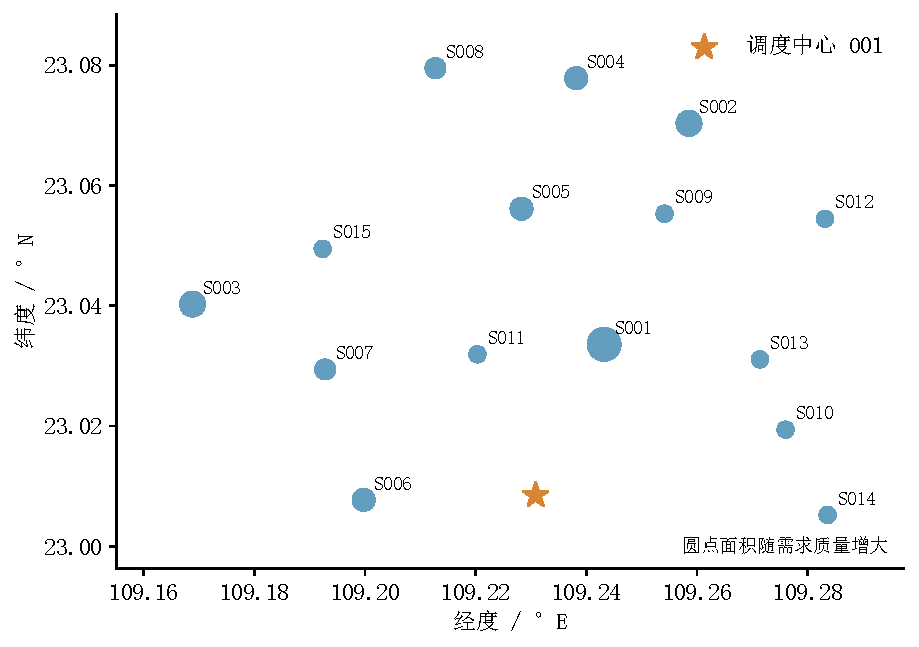
\includegraphics[width=.86\linewidth]{figures/data/raw_service_map.pdf}
\caption{调度中心与服务区分布：依据附件节点坐标与逐区需求绘制}
\label{fig:service-map}\end{figure}

\subsection{需求结构与时限分类}
逐箱统计得到总质量758 kg、总体积2.011 m$^3$。其中医疗箱16箱，首批保障箱30箱，二者交集15箱，故具有至少一种硬时限要求的货箱数为
\begin{equation}N_{hard}=16+30-15=31.\label{eq:hard-count}\end{equation}
余下49箱使用期望送达时间计算软迟到。交集不能重复计数：同一货箱既为医疗物资又为首批保障时，应取两个适用截止时刻的较小值，而不是将其视为两项配送任务。

图\ref{fig:demand}同时展示需求质量和硬软时限构成。这一组合图把载荷规模与时间紧迫程度并列，便于识别“质量较大”与“必须尽早送达”并非同一概念。图\ref{fig:deadlines}进一步区分仅医疗、仅首批、两者兼有和一般物资；相同坐标的样本合并表示，避免重叠掩盖数量。

从逐区统计可见，S001拥有15箱、154 kg需求，约占总质量的20.3\%；S009至S015各有3箱、25 kg需求。S001的硬时限箱为3箱，其余服务区均为2箱，说明需求质量的差异明显大于硬时限箱数量的差异。调度时需要既给各区配置早期保障，又为大需求节点安排后续运力，不能仅按总质量大小排序服务。
\begin{figure}[htbp]\centering
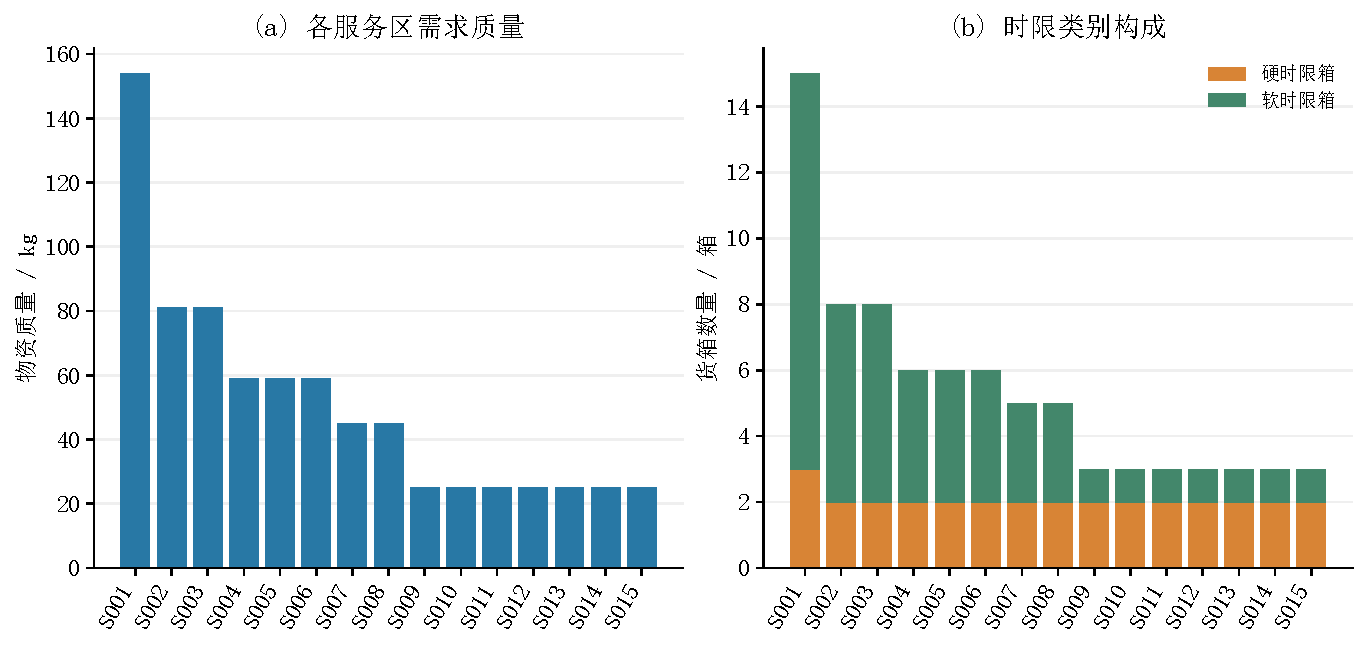
\includegraphics[width=\linewidth]{figures/data/raw_demand_composition.pdf}
\caption{各服务区的需求质量及硬软时限货箱构成}\label{fig:demand}\end{figure}
\begin{figure}[htbp]\centering
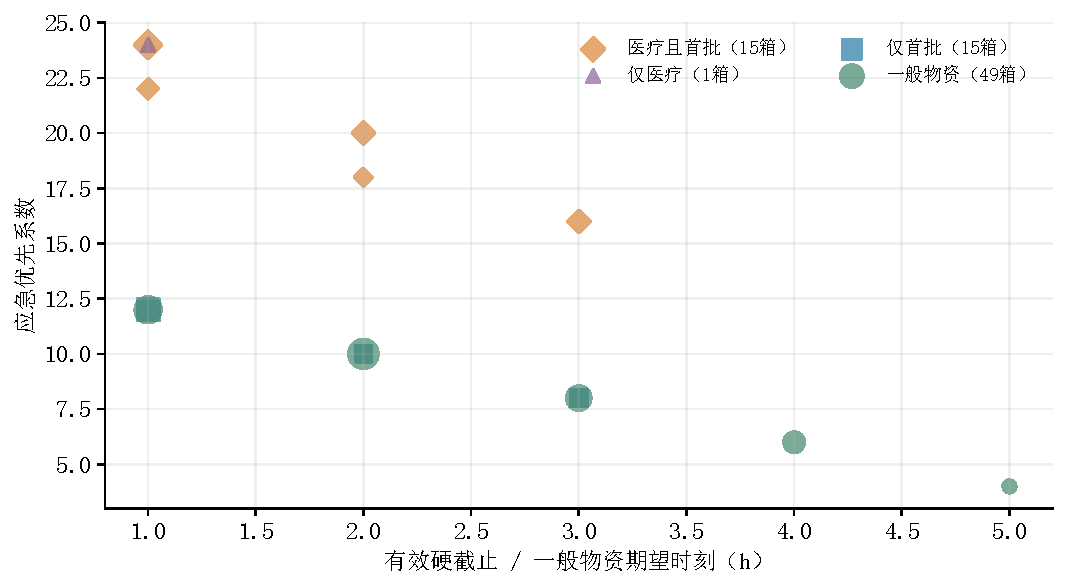
\includegraphics[width=.9\linewidth]{figures/data/raw_deadline_classes.pdf}
\caption{时限与优先系数：硬时限箱采用有效截止，一般物资采用期望时刻；点面积随同坐标箱数增大}\label{fig:deadlines}\end{figure}

\subsection{异构机型与能源库存}
三类机型的容量和库存见表\ref{tab:types}。C型具有较大的额定载质量和体积，但不能仅凭容量判定其在所有节点最优：不同载荷下的等效航程、爬升质量和实体数量均会影响调度。共享电池总数包含初始装机与备用电池，不能再额外加上实体机数量。
\begin{table}[htbp]\centering
\caption{运输机型容量与同型资源库存}\label{tab:types}
\begin{tabular}{lrrrrr}\toprule
机型 & 载质量/kg & 体积/m$^3$ & 能量/kWh & 实体机/架 & 电池/组\\\midrule
A & 25 & 0.060 & 4.5 & 4 & 6\\
B & 30 & 0.073 & 4.0 & 2 & 4\\
C & 80 & 0.250 & 8.0 & 2 & 4\\\bottomrule
\end{tabular}\end{table}

\subsection{航段、地形净空与飞行时间}
设节点经纬度为$(\lambda_i,\varphi_i)$，采用局部米制近似计算节点对距离：
\begin{equation}
d_{ij}=R\sqrt{\cos^2\!\left(\frac{\varphi_i+\varphi_j}{2}\right)(\lambda_j-\lambda_i)^2+(\varphi_j-\varphi_i)^2},
\end{equation}
其中角度以弧度计，$R=6371008.8$ m。该距离只对应水平巡航段；垂直运动在飞行时间中分别计算。

令$\mathcal C_{ij}$为航段水平直线实际经过的DEM像元集合，$H_c$为像元地面高程。题设要求的巡航海拔为
\begin{equation}
H_{ij}^{c}=\max_{c\in\mathcal C_{ij}}H_c+50.\label{eq:terrain}
\end{equation}
计算时应按地理配准及像元边界确定$\mathcal C_{ij}$，覆盖短距离穿越的像元；固定步长采样点的最大值并不天然等于经过像元的最大值。此处给出模型定义，具体像元遍历和边界处理仍需按该定义复验。

调度中心作业海拔为给定地面海拔，服务区作业海拔为地面海拔加30 m。由此定义
\begin{equation}
h_{ij}^{+}=\max(0,H_{ij}^{c}-H_i^{op}),\qquad
h_{ij}^{-}=\max(0,H_{ij}^{c}-H_j^{op}).
\end{equation}
每一航段的时间均为爬升、水平巡航和下降时间之和：
\begin{equation}
t_{gij}=\frac{h_{ij}^{+}}{v_g^{up}}+\frac{d_{ij}}{v_g^{cr}}+\frac{h_{ij}^{-}}{v_g^{down}}.\label{eq:leg-time}
\end{equation}
多点任务在每次交付后从服务区作业高度重新爬升，不能将多个访问点之间的飞行简化为一次长距离等高巡航。

\subsection{载荷相关能耗与返航约束}
附件的等效航程随当前载荷变化：
\begin{equation}
L_g(q)=L_g^0-(L_g^0-L_g^F)\left(\frac{q}{Q_g}\right)^{3/2},\quad 0\le q\le Q_g.
\label{eq:range}
\end{equation}
按前述能耗解释，水平航段能耗和爬升附加能耗分别为
\begin{equation}
E_{gij}^{hor}(q)=E_g^{use}\frac{d_{ij}}{L_g(q)},\qquad
E_{gij}^{up}(q)=\frac{(m_g^0+q)g_0h_{ij}^{+}}{3.6\times10^6\eta_g^{up}}.
\label{eq:energy}
\end{equation}
式中$g_0=9.80665$ m/s$^2$，分母$3.6\times10^6$把焦耳换算为kWh。下降效率取0时，不另计下降附加能耗，也不作能量回收。货箱交付后，从剩余载荷中扣除其质量；返航通常为空载，不能把起飞载荷代入整个架次。

架次$r$的总能耗和返航荷电状态满足
\begin{equation}
E_r=\sum_{(i,j)\in r}\bigl(E_{gij}^{hor}(q_{ij})+E_{gij}^{up}(q_{ij})\bigr),
\quad SOC_r^{end}=1-\frac{E_r}{E_g^{use}}\ge\rho_g.
\label{eq:soc}
\end{equation}

\subsection{两阶段充电与资源再次可用}
令返航SOC为$s$，从$s$充至满电所需时间按题面规则计算：
\begin{equation}
T^{chg}(s)=T^{full}\begin{cases}
0.65(0.9-s)/0.9+0.35,&0\le s<0.9,\\
0.35(1-s)/0.1,&0.9\le s\le1.
\end{cases}\label{eq:charge}
\end{equation}
该式在$s=0.9$处连续，在$s=1$时为0。每组电池返航后单独记录SOC和充电结束时刻，同型电池可在不同实体机之间调配，异型电池不得混用。不同能源资源可以并行充电，因此在未给出充电工位限制的条件下，不额外引入单工位排队。

\section{问题一：单点往返运输能力与货箱组批}
\subsection{分析思路与安全载荷边界}
单点任务限定为O01到服务区再返回O01，去程载货、返程空载。其决策可以分成两层：先判断机型在该节点的能量允许载荷，再决定哪些完整货箱组成一个批次。前者是连续质量变量问题，后者是离散集合划分问题，不能用最大安全载荷直接除总需求代替组批。

定义机型$g$服务节点$i$的往返能耗函数
\begin{equation}
F_{gi}(q)=E_{g,O01,i}(q)+E_{g,i,O01}(0),\qquad B_g=(1-\rho_g)E_g^{use}.
\end{equation}
在给定机型空载航程不小于满载航程、爬升效率为正时，$F_{gi}(q)$对$q$非减。因此最大安全载荷按以下边界处理：
\begin{equation}
q_{gi}^{safe}=\begin{cases}
\text{不可达},&F_{gi}(0)>B_g,\\
Q_g,&F_{gi}(Q_g)\le B_g,\\
\sup\{q\in[0,Q_g]:F_{gi}(q)\le B_g\},&\text{其他情况}.
\end{cases}\label{eq:safe-payload}
\end{equation}
最后一种情况可用二分求解，维护可行下界与不可行上界，直到区间宽度达到所需精度。空载不可达应单独标记，不能输出0 kg并把该机型保留为可行运输选择。即使安全载荷达到额定上限，实际组批仍可能首先受到体积约束。

\subsection{可行子集与多指标代价}
设$B_i$为服务区$i$的货箱集合。对每个非空子集$S\subseteq B_i$和机型$g$，计算总质量$w(S)$、总体积$v(S)$和往返能耗，保留满足
\begin{equation}
w(S)=\sum_{b\in S}w_b\le Q_g,\quad
v(S)=\sum_{b\in S}v_b\le V_g,\quad F_{gi}(w(S))\le B_g
\end{equation}
的候选$(S,g)$。其作业时间包含准备、逐箱装载、往返飞行及投送交接：
\begin{equation}
T(S,g)=t_g^{prep}+|S|t_g^{load}+t_{g,O01,i}
+t_g^{base}+|S|t_g^{handover}+t_{g,i,O01}.
\end{equation}
本文优先减少架次数，以降低独立执行任务数；架次数相同时减少能耗，再比较累计作业时间。相应的候选代价向量为
\begin{equation}c(S,g)=\bigl(1,F_{gi}(w(S)),T(S,g)\bigr).\end{equation}
这是明确的字典序偏好，而不是把不同量纲的指标直接相加。若应急管理者更重视时间，可以改变优先顺序，但必须重新求解并报告由此产生的取舍。

\subsection{集合划分动态规划}
令$D(M)$为覆盖货箱子集$M$的最优代价向量，$D(\varnothing)=(0,0,0)$。从$M$中取编号最小的货箱$b_*(M)$，则递推为
\begin{equation}
D(M)=\lexmin_{\substack{(S,g)\text{可行},\ S\subseteq M\\b_*(M)\in S}}
\{D(M\setminus S)+c(S,g)\}.\label{eq:dp}
\end{equation}
要求候选包含$b_*(M)$仅消除同一划分的排列重复，不删去合法划分。回溯递推选择即可获得每个批次的货箱集合与机型。各服务区分别求解，在问题一不设跨区资源耦合的条件下，将局部结果合并即得到全场景组批。

图\ref{fig:q1-flow}概括求解流程。对节点拥有$n_i$箱的情况，子集枚举规模为$2^{n_i}$，朴素子集递推量级为$3^{n_i}$；适合逐服务区的小规模离散问题，但不宜把全部80箱合成一个位掩码问题。
\begin{figure}[htbp]\centering
\begin{tikzpicture}[node distance=8mm]
\node[block,text width=11cm] (a) {节点坐标、经过像元的最高高程、机型参数、该区货箱};
\node[block,text width=11cm,below=of a] (b) {空载/满载边界判定，必要时二分求最大安全载荷};
\node[block,text width=11cm,below=of b] (c) {枚举子集与机型，筛选质量、体积和返航能量均可行的批次};
\node[block,text width=11cm,below=of c] (d) {集合划分动态规划：架次数优先，其次能耗，再次作业时间};
\node[block,text width=11cm,below=of d] (e) {回溯货箱与机型；复核逐箱覆盖、容量、能量与指标合计};
\draw[edge](a)--(b);\draw[edge](b)--(c);\draw[edge](c)--(d);\draw[edge](d)--(e);
\end{tikzpicture}
\caption{单点运输能力与货箱组批求解流程}\label{fig:q1-flow}
\end{figure}

\subsection{结果的检验与解释口径}
后续应按“15个节点乘3种机型”报告45项安全载荷，并对最终每个架次重新计算货箱质量、体积、往返能耗和作业时间。逐箱覆盖次数须恰为1，不允许遗漏、重复或跨区组批。安全载荷曲线与返航余量相联系，组批结果则用架次数、质量利用率和体积利用率解释。

本节确立模型和求解步骤，不给出尚未完成地形复核后的载荷与架次数值。关于安全余量的敏感性，应在每个余量水平重新生成可行候选并运行动态规划，不能只调整旧解的能耗门限后继续沿用原批次。

\section{问题二：异构无人机多点多架次运输调度}
\subsection{决策表示与硬软时限}
将运输架次$r$表示为机型$g_r$、访问序列$\pi_r$、货箱集合$B_r$、实体机$u_r$、共享电池$k_r$及准备开始时刻$s_r$。每个货箱必须恰属于一个架次，并在自身目的服务区交付；机型与实体机、电池类型必须匹配。

对医疗箱和首批保障箱定义适用截止集合$\mathcal D_b$：医疗箱加入期望时刻，首批箱加入首批截止。硬时限箱满足
\begin{equation}d_b^{hard}=\min\mathcal D_b,\qquad C_b\le d_b^{hard}.\end{equation}
对$\mathcal D_b=\varnothing$的软时限箱，仅在目标中评价归一化加权迟到：
\begin{equation}
WTD=\sum_{b\in B^{soft}}\alpha_b\frac{\max(0,C_b-d_b^{exp})}{d_b^{exp}}.\label{eq:wtd}
\end{equation}
这里的“送达”采用完成该箱交接的时刻$C_b$，并非无人机到达服务区的时刻。这样的区分在同站多箱交接时会影响临界货箱是否逾期。

\subsection{逐站时刻与剩余载荷递推}
令$\pi_r=(i_1,\ldots,i_m)$，$i_0=O01$，起飞时刻为
\begin{equation}\tau_{r0}^{dep}=s_r+t_{g_r}^{prep}+|B_r|t_{g_r}^{load}.\end{equation}
到达第$j$个服务区、完成站内投送和离开的时刻依次为
\begin{align}
\tau_{rj}^{arr}&=\tau_{r,j-1}^{dep}+t_{g_r,i_{j-1},i_j},\\
C_b&=\tau_{rj}^{arr}+t_{g_r}^{base}+\ell_b t_{g_r}^{handover},\\
\tau_{rj}^{dep}&=\tau_{rj}^{arr}+t_{g_r}^{base}+|B_{ri_j}|t_{g_r}^{handover}.
\end{align}
其中$\ell_b$为货箱在该站的交接序号。按有效硬截止升序、应急优先系数降序、编号升序排列，软时限箱在硬时限箱后依上述规则交接。离站后扣除本次交付质量，再用新的剩余载荷计算下一航段能耗。末站离开后加返航时间，得到$\tau_r^{ret}$。

这一递推把访问顺序同时作用于时间和能耗：较早卸下重箱可减轻后续载荷，但可能推迟其他节点的硬时限箱。多点路线必须逐段重算，不能仅在两个单点能耗之间做距离修正。

\subsection{实体机与电池的双资源约束}
运输实体机在半开区间$[s_r,\tau_r^{ret})$被占用；电池还需完成返航后的充电，因此其占用区间为
\begin{equation}I_r^{bat}=[s_r,\tau_r^{ret}+T^{chg}(SOC_r^{end})).\end{equation}
对每个实体机$u$和电池$k$，同一时刻分别满足
\begin{equation}
\sum_{r:u_r=u}\ind_{[s_r,\tau_r^{ret})}(t)\le1,\qquad
\sum_{r:k_r=k}\ind_{I_r^{bat}}(t)\le1.
\end{equation}
半开区间使“上一任务结束的瞬间开始下一任务”不会被重复计为冲突。题面未另给运输机周转时长，实体机返回后可开始准备；其原电池仍在充电时，可以换用已经满电的同型电池。

图\ref{fig:q2-resource}用符号时刻说明两类资源的差异。机体可再次执行并不意味着原电池可再次使用；这也是仅按无人机架数排列甘特图不足以检验资源可行性的原因。
\begin{figure}[htbp]\centering
\begin{tikzpicture}[x=.8cm,y=1cm,font=\small]
\draw[edge](0,0)--(13,0) node[right]{时间};
\node[anchor=east] at(0,1.2){实体机};\node[anchor=east]at(0,2.3){电池};
\filldraw[fill=blue!12,draw=blue!50] (1,.8) rectangle (7,1.6);
\node at(4,1.2){准备、飞行、交付与返航};
\filldraw[fill=blue!12,draw=blue!50] (1,1.9) rectangle (7,2.7);
\filldraw[fill=orange!15,draw=orange!60] (7,1.9) rectangle (12,2.7);
\node at(4,2.3){执行任务};\node at(9.5,2.3){返航后充电};
\foreach \x in {1,7,12}{\draw[dashed,gray](\x,0)--(\x,2.8);}
\node[below]at(1,0){$s_r$};\node[below]at(7,0){$\tau_r^{ret}$};
\node[below]at(12,0){$\tau_r^{ret}+T^{chg}$};
\end{tikzpicture}
\caption{运输机与共享电池占用差异示意；横向长度不代表实际计算时长}\label{fig:q2-resource}
\end{figure}

\subsection{求解流程与指标权衡}
在全部硬约束成立的集合内，以$(WTD,C_{max},E_T,N_T)$作为分层比较指标，其中
\begin{equation}C_{max}=\max_r\tau_r^{ret},\quad E_T=\sum_rE_r,\quad N_T=|\mathcal R|.\end{equation}
先保证医疗与首批交付，再比较一般物资及时性；在及时性相同的候选中依次减少完工时间、能耗和架次数。该目标定义评价偏好，并不意味着构造算法已经穷尽其可行集合。

求解先用硬时限箱构造零违约基线并确定紧迫批次的实体机指派，随后枚举同一服务区普通货箱的补入组合。补入后的架次必须重新核验质量、体积、逐段递减载荷能耗、返航余量及每个硬时限，并保持硬时限箱优先交接。剩余货箱再执行单服务区精确组批和两服务区串访配对，最后由事件仿真器统一重排实体机与满电电池。算法同时保留硬箱专送基线，只有混装方案按$(N_{late}^{hard},WTD,C_{max},E_T,N_T)$字典序严格改进时才采用。

基于修正后的DEM穿越像元高程口径，表~\ref{tab:q2-compare}给出两套构造方案的实算比较。两者均完成80箱唯一交付，31箱硬时限货箱均无违约；混装方案把普通物资超期箱数由23箱降至9箱，并同时减少架次、完成时间和能耗，故选作问题二当前方案。
\begin{table}[htbp]
  \centering
  \caption{问题二基线与硬软混装方案比较}
  \label{tab:q2-compare}
  \begin{tabular}{lrrrrrr}
    \toprule
    方案 & 硬违约/箱 & 普通超期/箱 & $WTD$ & $C_{max}$/h & $E_T$/kWh & 架次 \\
    \midrule
    硬箱专送基线 & 0 & 23 & 111.492 & 3.527 & 83.012 & 26 \\
    硬软混装方案 & 0 & 9 & 38.787 & 2.679 & 69.602 & 22 \\
    \bottomrule
  \end{tabular}
\end{table}

相对基线，混装方案的$WTD$下降65.2\%，全部返航完成时间缩短24.1\%，总运输能耗下降16.2\%，架次下降15.4\%。这些指标来自确定性可行构造，不据此声称全局最优；逐架次路线、逐箱完成时刻以及无人机和电池编号分别记录在结果表中。

\section{问题三：连续通信约束下的运输与中继协同}
\subsection{双向链路预算与可用性}
固定网关G01位于O01，通信端点海拔由地面海拔与天线离地高度确定；运输端点随爬升、巡航、下降和交接阶段变化。接收门限为灵敏度与衰落裕量之和，附件中相应值为
\begin{equation}P_{th}=P_{sens}+M=-98+8=-90\ \mathrm{dBm}.\end{equation}
对通信方向$a\to b$，允许传播损耗为
\begin{equation}
L_{a\to b}^{max}=P_t^a+G_t^a+G_r^b-L_{sys}-P_{th}^b,\qquad
L_{ab}^{max}=\min(L_{a\to b}^{max},L_{b\to a}^{max}).
\end{equation}
两个方向取小值，是因为指令下发与状态回传均须可用。将附件对应接口参数代入，可得运输机—网关、运输机—中继和中继—网关的双向预算分别为122、116和126 dB。这些是设备参数推导的门限，不是某条实际航迹的通信余量。

设$D_{ab}(t)$为端点三维直线距离，单位km；频率$f$以MHz计，附件2.4 GHz对应2400 MHz。传播损耗为
\begin{equation}
L_{ab}^{path}(t)=32.45+20\log_{10}f+20\log_{10}D_{ab}(t)+L_{obs}\beta_{abt}.
\end{equation}
其中$L_{obs}=10$ dB，遮挡变量由三维视线与沿途DEM比较确定。系统损耗已在预算侧扣除，不能在传播损耗侧再次扣减。定义
\begin{equation}
A_{ab}(t)=\ind\{L_{ab}^{path}(t)\le L_{ab}^{max}\},\quad
M_{ab}^{link}(t)=L_{ab}^{max}-L_{ab}^{path}(t).
\end{equation}
遮挡增加损耗，但不必然导致链路中断；最终仍须比较预算门限。

\subsection{合法通信拓扑与全时段服务}
图\ref{fig:q3-topology}给出题目允许的两种通信方式。直连不可用时，可以经同一架中继完成接入和回传，不允许通过多架中继接力跳转。
\begin{figure}[htbp]\centering
\begin{tikzpicture}
\node[block,text width=2.5cm] (t) at(0,0){运输无人机};
\node[block,text width=2.5cm] (r) at(5,0){在服中继};
\node[block,text width=2.5cm] (g) at(10,0){固定网关G01};
\draw[edge,<->](t)--node[above,font=\small]{接入链路}(r);
\draw[edge,<->](r)--node[above,font=\small]{回传链路}(g);
\draw[edge,<->](t.south)--++(0,-1.1)--node[below,font=\small]{直连链路}(10,-1.6)--(g.south);
\node[font=\small,align=center] at(5,1.4){中继模式要求接入与回传同时可用\\拓扑示意，不表示实际点位或覆盖范围};
\end{tikzpicture}
\caption{直连与单中继通信拓扑示意}\label{fig:q3-topology}
\end{figure}

令$\mathcal T_r$为运输架次需要保障的全部飞行与交接时刻，$I_h^{srv}$为中继$h$的在服区间。对任意$t\in\mathcal T_r$，要求
\begin{equation}
A_{rG}(t)=1\quad\text{或}\quad
\exists h:\ t\in I_h^{srv},\ A_{rh}(t)=1,\ A_{hG}(t)=1.
\label{eq:continuous}
\end{equation}
输出时优先标记直连；非直连时选择一架满足条件的中继，保证每时刻只有一个实际保障指派。允许多个中继在物理上可用，但不能由此把同一运输区间同时计作多项必要保障任务。

\subsection{中继悬停、能量与资源占用}
候选悬停点$p$须在DEM内，海拔为$H_p^R=H_p^{DEM}+h_p^{AGL}$，且$0<h_p^{AGL}\le300$ m。中继出航巡航海拔还要覆盖终点悬停海拔：
\begin{equation}
H_{O01,p}^{c}=\max\left(\max_{c\in\mathcal C_{O01,p}}H_c+50,\ H_p^R\right).
\end{equation}
出航按爬升、水平巡航、必要下降计算，返航同理。中继从准备开始到建链完成的时刻依次为
\begin{align}
\tau_h^{dep}&=s_h+t_R^{prep},&
\tau_h^{arr}&=\tau_h^{dep}+t_{O01,p}^{fly},\\
\tau_h^{link}&=\tau_h^{arr}+t_R^{link},&
\tau_h^{ret}&=\tau_h^{end}+t_{p,O01}^{fly}.
\end{align}
只有在$[\tau_h^{link},\tau_h^{end}]$内才能提供保障。总能耗写为
\begin{align}
E_h^{fly}&=\frac{P_R^{cr}}{3600}\left(\frac{d_{O01,p}}{v_R^{cr}}+\frac{d_{p,O01}}{v_R^{cr}}\right)
+\frac{m_Rg_0(h_{O01,p}^{+}+h_{p,O01}^{+})}{3.6\times10^6\eta_R^{up}},\\
E_h&=E_h^{fly}+\frac{(P_R^{hover}+P_R^{com})(\tau_h^{end}-\tau_h^{arr})}{3600}
\le(1-\rho_R)E_R^{use}.\label{eq:relay-energy}
\end{align}
功率以kW计，故时间需除以3600。这里把建链期间按悬停及通信功率计入能源消耗，明确计费从抵达开始，而服务可用从建链完成开始。

中继实体机占用$[s_h,\tau_h^{ret}+t_R^{turn})$；能源组件占用任务及返航后充电区间。两架中继机和六组能源组件均按实体编号分配，在同一波次内也须逐一预占，不能让多个任务同时选中尚未更新状态的同一资源。

\subsection{候选覆盖与联合调度方法}
先将运输任务展开为分段线性三维轨迹，识别直连不足的时空位置，再从服务区邻域、航段附近和DEM高点形成候选悬停集合。依次剔除越界、回传不足和往返能量不可行的点。离散轨迹样本上的覆盖关系可用于快速筛选，但最终须按式\eqref{eq:continuous}验证整段时间。

联合候选方案采用硬截止优先组织运输批次，并根据中继最早建链时刻、最长可服务时长和能源再可用时刻调整波次。比较指标为一般物资迟到、联合完成时间、总能耗和总架次，其中
\begin{equation}
C_{max}^{joint}=\max\!\left(\max_r\tau_r^{ret},\max_h\tau_h^{ret}\right),\quad
E^{joint}=\sum_rE_r+\sum_hE_h.
\end{equation}
完成时间取最后返航，不包含此后的充电及周转。硬时限与连续通信必须先满足；不能用较少的中继能耗补偿已发生的通信中断。

\subsection{连续性验证与结果表达}
固定时间网格不能排除相邻样本之间的短时中断。验证时，应在每个线性运动区间给出传播损耗上界：距离项在区间端点求上界，地形项采用扫掠视线与经过像元的关系获得保守判定；无法判定的区间进一步细分。区间达到细分阈值仍未被证明可用时，应标记为未通过证明，不将其自动视为可行，也不直接断言实际已经中断。

后续需将认证区间与额外加密采样对照，并输出运输架次、阶段、起止时刻、直连或中继状态及实际中继架次。通信状态图、最小链路余量与联合资源甘特图分别回答“何时由谁保障”“距离门限有多少余量”“资源能否按时在位”。本阶段不报告尚未基于复核后轨迹得到的零中断、余量或中继数量结论。

\section{问题四：固定联合方案下的任务分区与资源配置}
\subsection{不可拆任务块与合法分区}
问题四的输入是问题三已经确定的联合方案，不能通过重排访问顺序或移动任务时刻降低资源需求。以15个服务区为顶点，若某运输架次同时访问两个服务区，则在两顶点之间连边。同一连通分量内的服务区由共访关系直接或间接连接，必须作为不可拆的原子任务块。

设原子块集合为$\mathcal A=\{A_1,\ldots,A_m\}$，将其划分为$K=2$或3个非空组。令$x_{jk}\in\{0,1\}$表示原子块$j$归属组$k$，则
\begin{equation}
\sum_{k=1}^{K}x_{jk}=1\quad(j=1,\ldots,m),\qquad
\sum_{j=1}^{m}x_{jk}\ge1\quad(k=1,\ldots,K).
\end{equation}
若$m<K$，则该固定运输方案不支持要求的非空分区。原子块由实际路线决定，不能为了获得均衡地图而拆开共访服务区。

\subsection{从实际通信分段确定中继归属}
令$\mathcal R_k$为组$k$承担的运输架次集合，$\mathcal E$为问题三最终通信分段表中出现的“运输架次—中继架次”实际指派关系。该组所需中继任务为
\begin{equation}
\mathcal H_k=\{h:\exists r\in\mathcal R_k,\ (r,h)\in\mathcal E\}.
\label{eq:actual-relay}
\end{equation}
一架中继在某波次内在位，不意味着它实际保障了波次中所有运输任务。必须从通信分段的实际指派提取$\mathcal E$，而不能把整个波次的运输架次清单直接作为保障关系。

若同一中继任务属于多个$\mathcal H_k$，各相关组独立配置资源，并保留其完整悬停点和完整原任务时段。这样既保持题设任务安排不变，又避免把并未服务本组的中继任务错误计入本组。图\ref{fig:q4-flow}给出这一资源归属链。
\begin{figure}[htbp]\centering
\begin{tikzpicture}[node distance=8mm]
\node[block,text width=5.2cm](route)at(0,0){固定运输路线\\建立服务区共访图};
\node[block,text width=5.2cm](comm)at(6,0){最终通信分段\\提取实际运输—中继关系};
\node[block,text width=5.2cm,below=of route](atom){共访连通分量\\形成不可拆原子块};
\node[block,text width=5.2cm,below=of comm](relay){确定各组关联中继\\保留完整任务时段};
\node[block,text width=11.5cm](peak)at(3,-3.4){枚举合法分区；按类型计算无人机、能源资源占用区间峰值};
\node[block,text width=11.5cm,below=of peak](out){比较配置规模、相对集中执行的冗余、库存缺口与工作量均衡};
\draw[edge](route)--(atom);\draw[edge](comm)--(relay);
\draw[edge](atom)--(atom.south|-peak.north);\draw[edge](relay)--(relay.south|-peak.north);
\draw[edge](peak)--(out);
\end{tikzpicture}
\caption{固定方案分区与资源核算流程；不代表已求得的具体服务区分组}\label{fig:q4-flow}
\end{figure}

\subsection{固定时序的最小独立资源数}
对组$k$和资源类型$a$，设必须执行的占用区间集合为$\mathcal I_{ka}$。同型资源可互换、各任务时刻固定且没有额外资源专属约束时，最小配置数等于区间峰值并发数：
\begin{equation}n_{ka}=\max_t\sum_{I\in\mathcal I_{ka}}\ind_I(t).\label{eq:peak}\end{equation}
原因是任何同时占用的区间都必须使用不同实体；反过来，按开始时刻排序、结束后回收资源的贪心分配可用峰值数量完成所有区间。

对运输机按机型分别统计任务区间，对运输电池计入任务后的完整充电；对中继机计入周转，对能源组件计入充电。所有区间采用左闭右开约定，同一时刻结束事件优先于开始事件处理。若未来增加资源专属兼容性、共享充电工位或不同初始SOC，峰值数量不再自动构成充分条件，应扩展资源模型。

\subsection{库存缺口、冗余与组间均衡}
设$I_a$为全局库存，$n_a^{central}$为同一有效联合方案集中执行所需的资源，则
\begin{equation}
D_a^{(K)}=\max\left(0,\sum_kn_{ka}-I_a\right),\qquad
R_a^{(K)}=\sum_kn_{ka}-n_a^{central}.\label{eq:shortage}
\end{equation}
前者描述资源采购或增援缺口，后者描述分区独立执行相对集中执行新增的配置。不能让每个组分别减去一份完整全局库存，也不能把“库存剩余”称为分区冗余。

以组内运输机任务占用时长和中继机含周转的占用时长之和定义工作量$W_k$，不把能源充电时间再次计作无人机机时。均衡性采用总体标准差口径：
\begin{equation}
\bar W=\frac1K\sum_kW_k,\qquad
CV_W=\frac{\sqrt{K^{-1}\sum_k(W_k-\bar W)^2}}{\bar W}.
\end{equation}
另以各组最后返航时刻之差评价完成时间均衡。两者回答不同问题：机时相近的组仍可能因等待或晚开始而较晚结束。

\subsection{分区搜索与比较原则}
按固定顺序逐一分配原子块，并以首次出现的组编号规范化消除标签对称。在每个合法分区上构造$\mathcal R_k$及$\mathcal H_k$，由式\eqref{eq:peak}计算资源向量，再比较缺口、总配置数量、$CV_W$和组间完成时刻极差。跨类型合计仅表示“件数优先”的一种建模偏好，不代表不同资源采购价格相同；同时应完整报告分类型向量，以免合计掩盖资源差异。

在枚举完全部合法分区、且输入方案与资源关系正确的前提下，可以讨论固定问题三方案下的最优划分。本阶段尚不输出具体分区、资源最小值或缺口数值。后续结果图应同时给出分区地图与分类型资源表，以说明空间分组为何引起某类资源复制，而不是只展示颜色不同的区域。

\section{模型检验与敏感性分析设计}
\subsection{分层验证思路}
验证应沿模型依赖链展开。先确认航段经过像元、作业高度和能耗单位，再核对单架次计算，之后检验全局资源与通信。若公共地形函数存在偏差，即使输出表之间完全一致，也不能据此证明任务满足50 m净空。

单架次检查包含四项：货箱质量与体积、随交付递减的剩余载荷、逐站交接时刻、累计能耗与返航SOC。全方案再检查每箱只出现一次、全部硬截止满足、实体及能源区间不重叠。问题三在此基础上对每段轨迹给出连续通信依据；问题四则重建实际保障关系，核对分组前后的固定任务和时刻。

\subsection{敏感性实验的定义与解释边界}
表\ref{tab:validation-plan}给出后续实验设计。表中内容为计划检验的参数与指标，并不表示已完成对应实验。
\begin{table}[htbp]\centering
\caption{后续敏感性实验与验证设计}\label{tab:validation-plan}
\begin{tabularx}{\linewidth}{>{\raggedright\arraybackslash}p{2.5cm}YY}\toprule
实验对象 & 参数变化与重算范围 & 拟报告指标\\\midrule
返航余量 & 10\%、15\%、20\%、25\%、30\%；重算安全载荷与组批 & 各机型载荷、架次数、能耗、累计作业时间\\
地面操作延误 & 在单次装载、换电或交接事件中加入延误，并重跑调度 & 硬逾期箱数、WTD、完工时间与资源峰值\\
能耗不确定性 & 水平能耗系数及爬升效率分别扰动，先独立再联合比较 & 能量不可行架次、重新调度后的代价变化\\
链路保守余量 & 收紧允许传播损耗，重新认证并按需调整中继方案 & 认证未通过区间、调整后的能耗与完工时间\\
分区执行方式 & 主方案保持完整中继任务；局部时段裁剪仅作另行假设对照 & 分类型配置、缺口、冗余与均衡变化\\
\bottomrule\end{tabularx}\end{table}

返航余量增加会收缩可行载荷集合，但组批架次数可能呈阶梯变化。因此应同时展示连续载荷曲线和离散组批指标。地面延误不能仅用“全部交付时刻统一加常数”代替，因为每个事件的延误会沿同一实体机和共享电池的后续任务传播。

通信鲁棒性应区分“旧保守证据不再足以保证”与“实际链路中断”。直接从旧余量减去附加损耗只能做证据裕度筛查；若要声称鲁棒方案仍可行，必须重新执行区间验证，必要时重新选点和调度，并比较对应目标损失。

\subsection{图表与数值的一致性检查}
正式结果应由同一份逐架次、逐箱和通信分段数据生成，汇总指标可以逐项回算。每问结果至少回答一个明确问题：问题一说明容量瓶颈，问题二说明交付与资源时序，问题三说明连续保障与代价，问题四说明独立分区造成的资源变化。相同指标的比较图使用一致量纲和色标；示意图不承担数值验证功能。

附录\ref{app:outputs}列出后续结果表需要保留的字段。这些字段同时服务计算复核与图表解释，使“图上看到的现象”能够定位到具体架次、货箱或时间区间。

\section{方法评价与阶段性结论}
\subsection{模型的适用性与局限}
本文框架把单点能力、调度、中继和分区组织在同一套物理与资源定义之下。其可解释性来自对象层次的区分：货箱是交付最小单位，架次是飞行任务单位，实体机与电池是分别占用的资源，通信分段是实际保障关系的记录单位。这样可以定位容量不足、能源等待或中继复制的具体来源。

模型的精确性范围也具有层次。单点集合划分在候选完整时可精确求解；固定时序区间模型可精确核算资源数；多点运输和静态中继候选的联合构造仍受启发式与候选集合限制。即使连续通信检验通过，也只证明该方案满足指定传播判据，并不证明中继点位或整体目标达到全局最优。

实际救援还受到天气、定位误差、临时禁飞、充电设备条件和动态需求影响。当前模型采用附件确定参数，30米DEM不能表征全部小尺度障碍，题设传播公式也不是完整无线环境仿真。因此，得到的方案应理解为标准场景下的计划依据，其推广需要额外的气象、通信和装备实测数据。

\subsection{已经形成的认识与后续定量问题}
从原始附件可以确认，运输需求同时包含较大质量的物资与具有紧迫时限的货箱，31个硬时限箱必须优先进入可行性判断。由模型可知，单点最大安全载荷受额定质量、爬升能耗与返航余量共同限制，实际批次还可能受体积主导；多点调度则必须在逐站卸载和共享电池再可用之间进行时序协调。

通信约束使中继在位时间成为运输可行性的组成部分。任务分区进一步放大资源不可跨组共享的影响，而这种影响只能沿实际保障关系计算，不能用同波次关系替代。本稿已经给出上述问题的数学表达与检验路径，但最终载荷、调度指标、中继方案、分区配置以及敏感性数值尚需统一复算后补充，不据方法描述推断任何最终最优方案。

\bibliographystyle{unsrt}
\bibliography{references}
\clearpage
\appendix
\section{逐区需求与结果表口径}\label{app:outputs}
\subsection{逐服务区需求统计}
表\ref{tab:demand-details}依据逐箱清单汇总，硬时限箱按医疗与首批要求的并集计算。正文中的总质量、体积和31箱硬时限均可由该表回算。
\begin{longtable}{lrrrr}
\caption{逐服务区需求统计}\label{tab:demand-details}\\
\toprule 服务区 & 箱数 & 质量/kg & 体积/m$^3$ & 硬时限箱数\\\midrule\endfirsthead
\toprule 服务区 & 箱数 & 质量/kg & 体积/m$^3$ & 硬时限箱数\\\midrule\endhead
S001 & 15 & 154.00 & 0.394 & 3 \\
S002 & 8 & 81.00 & 0.211 & 2 \\
S003 & 8 & 81.00 & 0.211 & 2 \\
S004 & 6 & 59.00 & 0.156 & 2 \\
S005 & 6 & 59.00 & 0.156 & 2 \\
S006 & 6 & 59.00 & 0.156 & 2 \\
S007 & 5 & 45.00 & 0.129 & 2 \\
S008 & 5 & 45.00 & 0.129 & 2 \\
S009 & 3 & 25.00 & 0.067 & 2 \\
S010 & 3 & 25.00 & 0.067 & 2 \\
S011 & 3 & 25.00 & 0.067 & 2 \\
S012 & 3 & 25.00 & 0.067 & 2 \\
S013 & 3 & 25.00 & 0.067 & 2 \\
S014 & 3 & 25.00 & 0.067 & 2 \\
S015 & 3 & 25.00 & 0.067 & 2 \\
合计 & 80 & 758.00 & 2.011 & 31 \\
\bottomrule\end{longtable}


\subsection{逐箱、逐架次和通信分段的输出}
\begin{table}[H]\centering
\caption{结果记录的对象与关键字段}\label{tab:output-fields}
\begin{tabularx}{\linewidth}{p{2.6cm}Y}\toprule
记录对象 & 关键字段与解释\\\midrule
单点批次 & 服务区、货箱集合、机型、质量、体积、能耗、完整作业时长\\
运输架次 & 架次编号、访问顺序、机型、实体机、电池、准备开始、起飞、返航、能耗与SOC\\
逐箱交付 & 货箱编号、所属架次、服务区、站内交接序号、交付完成、硬截止或期望时刻\\
能源周转 & 能源编号、任务区间、返航SOC、充电开始和结束、下次分配任务\\
中继架次 & 悬停经纬度与海拔、离地高度、实体机、能源组件、抵达、建链、服务结束和返航\\
通信分段 & 运输架次、飞行或交接阶段、区间边界、直连或中继状态、实际中继编号、可用性依据\\
分区配置 & 服务区集合、关联运输及中继任务、分类型资源数、全局缺口、相对集中执行冗余与工作量\\
\bottomrule\end{tabularx}\end{table}

表\ref{tab:output-fields}中的“开始”统一指准备开始，“交付”指单箱交接完成，“任务完成”指最后返航。电池及能源组件的充电结束只用于下一任务可用性，不加入已完成任务的完工时间。完整求解源程序和最终结果文件在其计算口径复核后作为支撑材料另行整理。

\end{document}
